\documentclass[10pt]{article}

\usepackage[utf8]{inputenc}
\usepackage{latexsym,amsfonts,amssymb,amsthm,amsmath}
\setlength{\parindent}{0in}
\setlength{\parskip}{\baselineskip}
\setlength{\oddsidemargin}{0in}
\setlength{\textwidth}{6.5in}
\setlength{\textheight}{8.8in}
\setlength{\topmargin}{0in}
\setlength{\headheight}{18pt}

\usepackage[a4paper,margin=1in,footskip=0.25in]{geometry}

\usepackage{listings}
\usepackage{color} %red, green, blue, yellow, cyan, magenta, black, white
\definecolor{mygreen}{RGB}{28,172,0} % color values Red, Green, Blue
\definecolor{mylilas}{RGB}{170,55,241}

\usepackage{graphicx}
\graphicspath{{../output/}}

\def\code#1{\texttt{#1}}

\usepackage[colorlinks=true, urlcolor=blue, linkcolor=blue]{hyperref}

\usepackage{verbatim}

\title{PHYS 410 Project 1}
\author{Gavin Pringle, 56401938}

%%%%%%%%%%%%%%%%%%%%%%%%%%%%%%%%%%%%%%%%%%%%%%%%%%%%%%%%%%%%%%%%%%%%%%%%%%%%%%%%%%%%%%%%%%%%%%%%%%%%%%%
% Start of document
%%%%%%%%%%%%%%%%%%%%%%%%%%%%%%%%%%%%%%%%%%%%%%%%%%%%%%%%%%%%%%%%%%%%%%%%%%%%%%%%%%%%%%%%%%%%%%%%%%%%%%%
\begin{document}

\maketitle

\lstset{language=Matlab,%
    %basicstyle=\color{red},
    breaklines=true,%
    morekeywords={matlab2tikz},
    keywordstyle=\color{blue},%
    morekeywords=[2]{1}, keywordstyle=[2]{\color{black}},
    identifierstyle=\color{black},%
    stringstyle=\color{mylilas},
    commentstyle=\color{mygreen},%
    showstringspaces=false,%without this there will be a symbol in the places where there is a space
    numbers=left,%
    numberstyle={\tiny \color{black}},% size of the numbers
    numbersep=9pt, % this defines how far the numbers are from the text
    emph=[1]{for,end,break},emphstyle=[1]\color{red}, %some words to emphasise
    %emph=[2]{word1,word2}, emphstyle=[2]{style},    
}

%%%%%%%%%%%%%%%%%%%%%%%%%%%%%%%%%%%%%%%%%%%%%%%%%%%%%%%%%%%%%%%%%%%%%%%%%%%%%%%%%%%%%%%%%%%%%%%%%%%%%%%
% Introduction
%%%%%%%%%%%%%%%%%%%%%%%%%%%%%%%%%%%%%%%%%%%%%%%%%%%%%%%%%%%%%%%%%%%%%%%%%%%%%%%%%%%%%%%%%%%%%%%%%%%%%%%
\subsection*{Introduction}

In this project, the problem of $N$ identical point charges confined to free motion on the surface of a 
sphere is examined. Via a finite-difference approximation simulation, the dynamic behaviour of point 
charges each originating from random initial positions on the surface of the sphere is computed. 
Since like charges repel, if a velocity-dependent retarding force is present for each charge then it 
follows that all charges will eventually reach a stable equilibrium where the electrostatic potential
energy is minimized. 
 
Through examining the potential energy of these equilibrium configurations as well as conducting 
equivalence class analysis, the equilibrium configurations of the charges are cataloged and their
symmetry is characterized. The equilibrium configurations in this problem are described in detail 
in the \href{https://en.wikipedia.org/wiki/Thomson_problem}{Thomson problem}.

In order to test the validity of the numerical model constructed for this problem, convergence testing 
is also applied. This is done by simulating an identical scenario using multiple discretization levels,
and analyzing the level-to-level differences. This convergence testing allows us to determine to which
order our finite difference approximation is accurate.

\pagebreak

%%%%%%%%%%%%%%%%%%%%%%%%%%%%%%%%%%%%%%%%%%%%%%%%%%%%%%%%%%%%%%%%%%%%%%%%%%%%%%%%%%%%%%%%%%%%%%%%%%%%%%%
% Review of Theory
%%%%%%%%%%%%%%%%%%%%%%%%%%%%%%%%%%%%%%%%%%%%%%%%%%%%%%%%%%%%%%%%%%%%%%%%%%%%%%%%%%%%%%%%%%%%%%%%%%%%%%%
\subsection*{Review of Theory}

\subsubsection*{Equations of motion}

In this simulation, natural units are used for all variables. This allows equations to be simplified by
setting all masses and charges as well as the radius of the confining sphere centered at the origin
equal to 1: 
$$m_i = 1, \quad q_i = 1, \quad R = 1$$
Using Cartesian coordinates, the position of each charge is written as 
$$\mathbf{r}_i(t) \equiv [x_i(t), y_i(t), z_i(t)] \quad , \quad i = 1, 2, \dots, N,$$
where
$$r_i \equiv |\mathbf{r}_i| \equiv \sqrt{x_i^2 + y_i^2 + z_i^2} = 1 \quad , \quad i = 1, 2, \dots, N.$$
The separation vectors between charges can be computed using the following formulas:
$$\mathbf{r}_{ij} = \mathbf{r}_j - \mathbf{r}_i \,$$
$$r_{ij} = |\mathbf{r}_j - \mathbf{r}_i| \,$$
$$\hat{r}_{ij} \equiv \frac{\mathbf{r}_j - \mathbf{r}_i}{r_{ij}} = \frac{\mathbf{r}_{ij}}{r_{ij}} \,.$$
The variable $\gamma$ is used as the scaling parameter for the velocity-dependent retarding force. The 
equation for Newton's second law can then be written for each charge as:
$$m_i a_i = F_{i, \textrm{electrostatic}} + F_{i, \textrm{retarding}}$$
which can be expanded to 
$$m_i \mathbf{a}_i=-k_e \sum_{j=1, j \neq i}^N \frac{q_i q_j}{r_{i j}} 
\hat{\mathbf{r}}_{i j}-\gamma \mathbf{v}_i, \quad i=1,2, \ldots N, \quad 0 \leq t \leq t_{\max }.$$
Using natural units ($k_e=1$) and writing $\mathbf{a}_i$ and $\mathbf{v}_i$ as derivatives of 
$\mathbf{r}_i$, this expression can be simplified to 
\begin{equation}\label{EOM}
\frac{d^2 \mathbf{r}_i}{d t^2}=-\sum_{j=1, j \neq i}^N \frac{\mathbf{r}_{i j}}{r_{i j}{ }^3}-\gamma 
\frac{d \mathbf{r}_i}{d t}, \quad i=1,2, \ldots N, \quad 0 \leq t \leq t_{\max }.
\end{equation}
The above equation is what is used to numerically solve the equations of motion using FDAs. 

\subsubsection*{Electrostatic Potential Energy}

The electrostatic potential energy of a point charge distribution is given by the following formula:
$$W=k_e \sum_{i=1}^N \sum_{j>i}^N \frac{q_i q_j}{r_{i j}}$$
Writing this potential energy in natural units and as a function of time, we can rewrite the above 
equation as:
\begin{equation}\label{potential}
V(t)=\sum_{i=2}^N \sum_{j=1}^{i-1} \frac{1}{r_{i j}}
\end{equation}
Since in our scenario energy is not conserved (kinetic energy is dissipated via the velocity-dependent
retarding force), we expect the potential to trend towards a minimum as $t \rightarrow \infty$.

\subsubsection*{Equivalence Classes}

The concept of \textit{equivalence classes} is introduced in order to characterize the different
equilibrium configurations of the point charges on the unit sphere. As $t \rightarrow \infty$ and 
$V$ is minimized, the equilibrium configuration for $N$ charges becomes independent of the initial
conditions. In words, the number of equivalence classes is the number of groups of charges that are 
indistinguishable in the equilibrium configuration. 

In order to calculate the number of equivalence classes, the magnitude of the displacement vector 
from charge $i$ to charge $j$ is defined as 
$$d_{i j}=\left|\mathbf{r}_j-\mathbf{r}_i\right| \quad i, j=1,2, \ldots, N$$
For charges $i$ and $i'$ in the same equivalence class, the lists of magnitudes $d_{i j}$ and 
$d_{i' j}$ to every other charge $j$ are the same.

%%%%%%%%%%%%%%%%%%%%%%%%%%%%%%%%%%%%%%%%%%%%%%%%%%%%%%%%%%%%%%%%%%%%%%%%%%%%%%%%%%%%%%%%%%%%%%%%%%%%%%%
% Numerical approach
%%%%%%%%%%%%%%%%%%%%%%%%%%%%%%%%%%%%%%%%%%%%%%%%%%%%%%%%%%%%%%%%%%%%%%%%%%%%%%%%%%%%%%%%%%%%%%%%%%%%%%%
\subsection*{Numerical Approach}

\subsubsection*{Finite Difference Equations}

For this assignment, the following second-order accurate FDAs are used for the first and second vector
time derivatives: 
\begin{equation}\label{first_derivative}
\left.\frac{d \mathbf{r}_i}{d t}\right|_{t=t^n} 
\rightarrow \frac{\mathbf{r}_i^{n+1}-\mathbf{r}_i^{n-1}}{2 \Delta t}
\end{equation}
\begin{equation}\label{second_derivative}
\left.\frac{d^2 \mathbf{r}_i}{d t^2}\right|_{t=t^n} 
\rightarrow \frac{\mathbf{r}_i^{n+1}-2 \mathbf{r}_i^n+\mathbf{r}_i^{n-1}}{\Delta t^2}
\end{equation}
with $t^n$ and $\Delta t$ defined as 
$$ \textrm{Total number of time steps:} \quad n_t=2^{\ell}+1 $$
$$ \textrm{Time step length:} \quad \Delta t=\frac{t_{\max }}{n_t-1}=2^{-\ell} t_{\max } $$
$$ \textrm{Time at time step } n: \quad t^n=(n-1) \Delta t, \quad n=1,2, \ldots n_t $$
Plugging (\ref{first_derivative}) and (\ref{second_derivative}) into (\ref{EOM}), we can create a new
FDA for the equations of motion (evaluated at time $t^n$):
$$ \frac{\mathbf{r}_i^{n+1}-2 \mathbf{r}_i^n+\mathbf{r}_i^{n-1}}{\Delta t^2} 
=\left.-\sum_{j=1, j \neq i}^N \frac{\mathbf{r}_{i j}}{r_{i j}{ }^3}\right|_{t=t^n}-
\gamma \frac{\mathbf{r}_i^{n+1}-\mathbf{r}_i^{n-1}}{2 \Delta t} $$
This equation can be reorganized to produce a formula for $\mathbf{r}_i^{n+1}$, the next position vector
following $\mathbf{r}_i^n$:
$$ \mathbf{r}_i^{n+1} = \left( \frac{1}{\Delta t^2} + \frac{\gamma}{2\Delta t} \right)^{-1} 
\left( \left( \frac{\gamma}{2\Delta t} - \frac{1}{\Delta t^2} \right) \mathbf{r}_i^{n-1} +
\frac{2}{\Delta t^2} \mathbf{r}_i^n \left.-\sum_{j=1, j \neq i}^N \frac{\mathbf{r}_{i j}}{r_{i j}{ }^3}
\right|_{t=t^n} \right) $$
In this implementation, the current time step $n$ is treated as the time step to be calculated, 
producing the following equation which is implemented in code:
\begin{equation}\label{FDA}
\mathbf{r}_i^{n} = \left( \frac{1}{\Delta t^2} + \frac{\gamma}{2\Delta t} \right)^{-1} 
\left( \left( \frac{\gamma}{2\Delta t} - \frac{1}{\Delta t^2} \right) \mathbf{r}_i^{n-2} +
\frac{2}{\Delta t^2} \mathbf{r}_i^{n-1} \left.-\sum_{j=1, j \neq i}^N \frac{\mathbf{r}_{i j}}{r_{i j}{ }^3}
\right|_{n-1} \right) 
\end{equation}

Since this FDA is a vector equation, it is evaluated three times for each charge at every time step for
each of the three Cartesian coordinate directions. Luckily, MATLAB syntax allows a vector equation such
as this one to be computed simultaneously for each coordinate. 

Additionally, since this FDA does not constrain charges to be on the unit sphere, each charge is 
re-normalized after by dividing its position by its magnitude:
\begin{equation}\label{normalization}
\tilde{\mathbf{r}}_i^n \rightarrow \frac{\mathbf{r}_i^n}{\left|\mathbf{r}_i^n \right|}=
\frac{\left[x_i^n, y_i^n, z^n\right]}
{\sqrt{\left(x_i^n\right)^2+\left(y_i^n\right)^2+\left(z_i^n\right)^2}}
\end{equation}
This normalization assumes that the distance the FDA (\ref{FDA}) moves each charge radially off the 
unit sphere is negligible.

\subsubsection*{Convergence Testing}

The validity of the FDA computed can be evaluated by conducting convergence analysis. Convergence 
analysis assumes that the error between the true solution and the computed solution is given by a 
\textit{function} $e_2(t^n)$ scaled by the time-step duration:
$$ \lim_{\Delta t\to 0} u_*(t^n) - u(t^n) \approx \Delta t e_2(t^n) 
\quad , \quad \textrm{If the approximation is first order}$$
$$ \lim_{\Delta t\to 0} u_*(t^n) - u(t^n) \approx \Delta t^2 e_2(t^n) 
\quad , \quad \textrm{If the approximation is second order}$$
where $u_*(t^n)$ is the true solution at each time step and $u(t^n)$ is the computed solution at 
each time step. 

Convergence analysis is done by computing the FDA for each time-step at different discretization levels 
$l$ and comparing the results. For a first order approximation this looks like 
$$du_l = u_l(t^n)-u_{l+1}(t^n) \approx -\frac{1}{2} \Delta t_l e_2(t^n)$$
$$du_{l+1} = u_{l+1}(t^n)-u_{l+2}(t^n) \approx -\frac{1}{4} \Delta t_l e_2(t^n)$$
For a second order approximation this looks like 
$$du_l = u_l(t^n)-u_{l+1}(t^n) \approx -\frac{3}{4} \Delta t_l^2 e_2(t^n)$$
$$du_{l+1} = u_{l+1}(t^n)-u_{l+2}(t^n) \approx -\frac{3}{16} \Delta t_l^2 e_2(t^n)$$
Therefore, for a first order approximation we expect to have 
\begin{equation}\label{first_order}
du_{l+1} \approx \frac{du_l}{2^1} , \quad du_{l+2} \approx \frac{du_l}{2^2} ,
\quad du_{l+3} \approx \frac{du_l}{2^3} , \quad \ldots
\end{equation}
and for a second order approximation we expect to have 
\begin{equation}\label{second_order}
du_{l+1} \approx \frac{du_l}{4^1} , \quad du_{l+2} \approx \frac{du_l}{4^2} , 
\quad du_{l+3} \approx \frac{du_l}{4^3} , \quad \ldots
\end{equation}

In our implementation we are using second order FDA to compute both the first and second time 
derivatives of position so the per-step error is second order. However, since the number of steps to
get to $t_{max}$ varies like $\frac{1}{\Delta t}$, we expect the overall simulation to have first order
accuracy and therefore we expect to convergence of curves as described by (\ref{first_order}).

%%%%%%%%%%%%%%%%%%%%%%%%%%%%%%%%%%%%%%%%%%%%%%%%%%%%%%%%%%%%%%%%%%%%%%%%%%%%%%%%%%%%%%%%%%%%%%%%%%%%%%%
% Implementation
%%%%%%%%%%%%%%%%%%%%%%%%%%%%%%%%%%%%%%%%%%%%%%%%%%%%%%%%%%%%%%%%%%%%%%%%%%%%%%%%%%%%%%%%%%%%%%%%%%%%%%%
\subsection*{Implementation}

Refer to Appendix A for the full source code implementation of the simulation, including the finite-
difference approximation, electrostatic potential computation, and equivalence class computation.  

In order to generate random initial positions of charges for code development as well as in 
\code{plotv.m} and \code{survey.m}, x, y and z coordinates for each charge are first chosen at random
locations on $[-1,1]$. For each charge, its initial position vector $\mathbf{r}_i^0$ is then 
re-normalized after by dividing it by its magnitude. This is shown in the code snippet below:
\begin{verbatim}
% Generate nc random inital locations for charges
r0 = 2*rand(nc,3) - 1;
for i = 1:nc
    r0(i,:) = r0(i,:)/(norm(r0(i,:)));
end
\end{verbatim}

The equivalence classes are computed in the suggested way described in the project outline. First, a 
matrix \code{dij} is generated which for each index \code{(i, j)} holds the magnitude of the vector from 
$\mathbf{r}_i^{n_t}$ to $\mathbf{r}_j^{n_t}$. This is implemented in MATLAB via the line 
\code{dij(i, j) = norm(r(j,:,nt) - r(i,:,nt))} placed inside a nested for loop. Each row of this matrix is 
then sorted in ascending order, which is interpreted as the list of distances from charge $i$ to each other
charge sorted in ascending order. In order to find which charges have matching rows (meaning they are in 
the same equivalence class), a nested for loop is used that compares each row to each other row in 
\code{dij}, while keeping track of which rows have already been placed into an equivalence class and how 
many rows (or charges) are in each equivalence class. Refer to Appendix A for the full source code. 

Please refer to Appendices B, C, and D for the source code for \code{convtest.m}, \code{plotv.m}, and
\code{survey.m}, respectively.

%%%%%%%%%%%%%%%%%%%%%%%%%%%%%%%%%%%%%%%%%%%%%%%%%%%%%%%%%%%%%%%%%%%%%%%%%%%%%%%%%%%%%%%%%%%%%%%%%%%%%%%
% Results
%%%%%%%%%%%%%%%%%%%%%%%%%%%%%%%%%%%%%%%%%%%%%%%%%%%%%%%%%%%%%%%%%%%%%%%%%%%%%%%%%%%%%%%%%%%%%%%%%%%%%%%
\subsection*{Results}

Through gradual development of 

\subsubsection*{convtest.m output}

\begin{figure}[ht!]
\centering
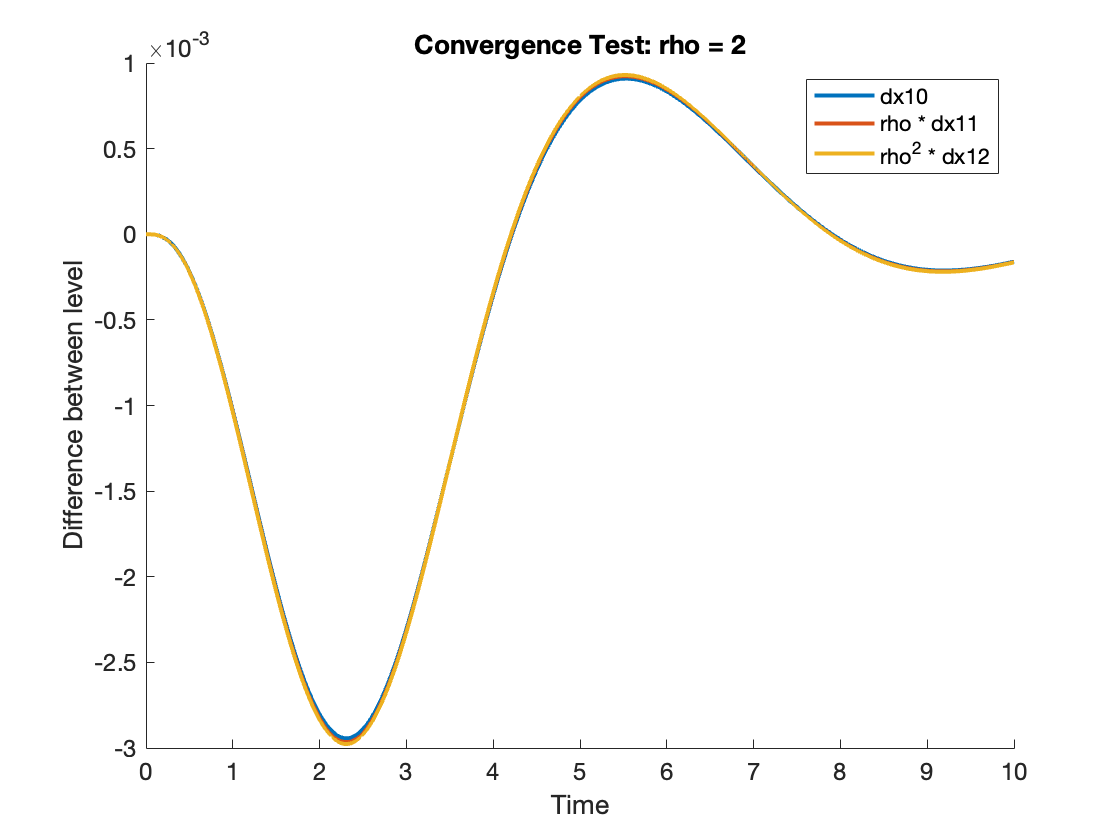
\includegraphics[width=0.75\textwidth]{ConvTest_2.png}
\caption{First order convergence test}
\end{figure}

\begin{figure}[ht!]
\centering
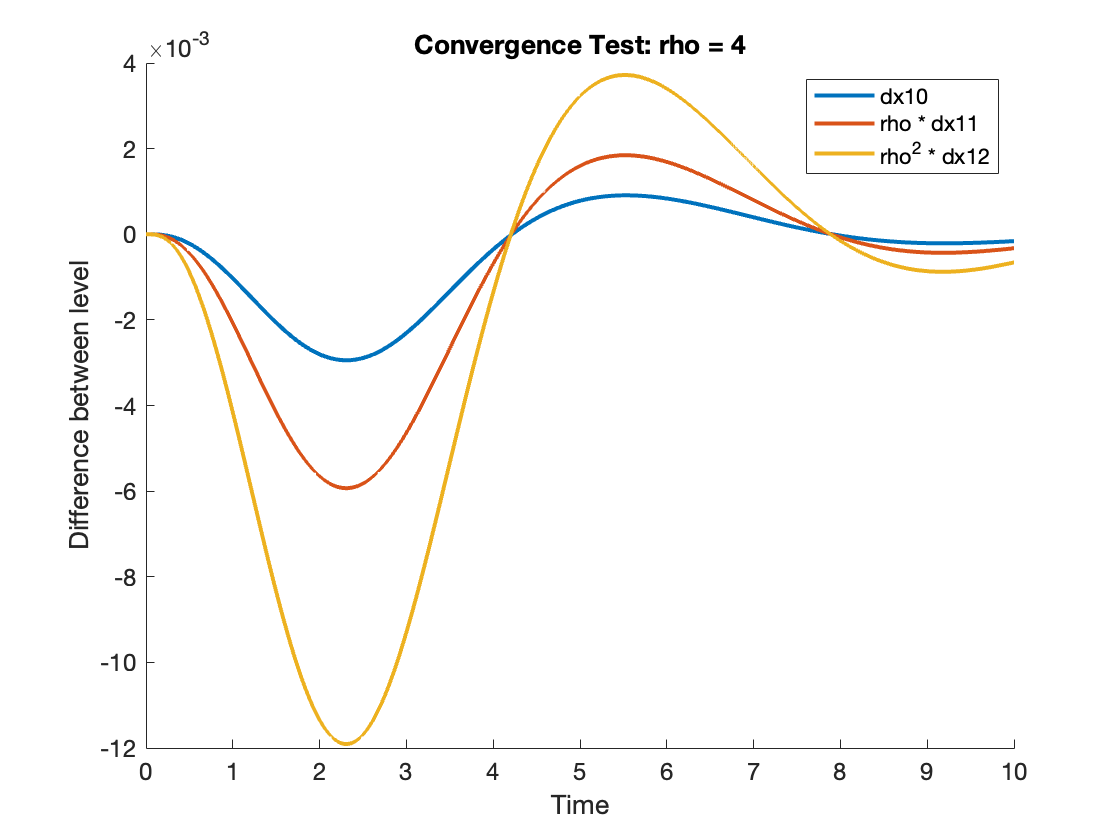
\includegraphics[width=0.75\textwidth]{ConvTest_4.png}
\caption{Second order convergence test}
\end{figure}

\subsubsection*{plotv.m output}

\begin{figure}[ht!]
\centering
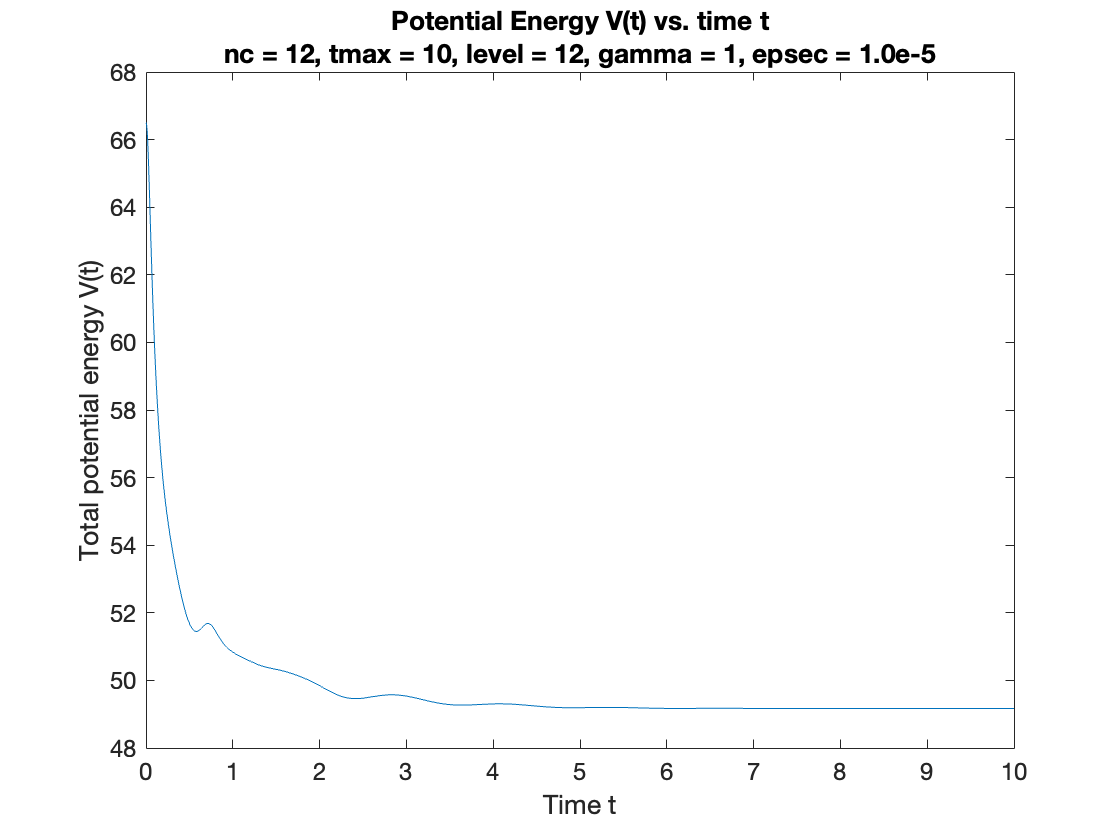
\includegraphics[width=0.75\textwidth]{plotv_output.png}
\caption{Output of \code{plotv.m} - electrostatic potential energy vs. time}
\end{figure}

\subsubsection*{survey.m output}

\verbatiminput{../output/vsurvey_GP.dat}
\verbatiminput{../output/ecsurvey_GP.dat}

\subsubsection*{Video of sample evolution}

The attached file \code{charges.mp4}

\pagebreak

%%%%%%%%%%%%%%%%%%%%%%%%%%%%%%%%%%%%%%%%%%%%%%%%%%%%%%%%%%%%%%%%%%%%%%%%%%%%%%%%%%%%%%%%%%%%%%%%%%%%%%%
% Conclusions
%%%%%%%%%%%%%%%%%%%%%%%%%%%%%%%%%%%%%%%%%%%%%%%%%%%%%%%%%%%%%%%%%%%%%%%%%%%%%%%%%%%%%%%%%%%%%%%%%%%%%%%
\subsection*{Conclusions}

% runtime shortcomings 

\pagebreak

%%%%%%%%%%%%%%%%%%%%%%%%%%%%%%%%%%%%%%%%%%%%%%%%%%%%%%%%%%%%%%%%%%%%%%%%%%%%%%%%%%%%%%%%%%%%%%%%%%%%%%%
% Appendix A - charges.m Code
%%%%%%%%%%%%%%%%%%%%%%%%%%%%%%%%%%%%%%%%%%%%%%%%%%%%%%%%%%%%%%%%%%%%%%%%%%%%%%%%%%%%%%%%%%%%%%%%%%%%%%%
\subsection*{Appendix A - charges.m Code}
\lstinputlisting{../src/charges.m}

\pagebreak

%%%%%%%%%%%%%%%%%%%%%%%%%%%%%%%%%%%%%%%%%%%%%%%%%%%%%%%%%%%%%%%%%%%%%%%%%%%%%%%%%%%%%%%%%%%%%%%%%%%%%%%
% Appendix B - convtest.m Code
%%%%%%%%%%%%%%%%%%%%%%%%%%%%%%%%%%%%%%%%%%%%%%%%%%%%%%%%%%%%%%%%%%%%%%%%%%%%%%%%%%%%%%%%%%%%%%%%%%%%%%%
\subsection*{Appendix B - convtest.m Code}
\lstinputlisting{../src/convtest.m}

\pagebreak

%%%%%%%%%%%%%%%%%%%%%%%%%%%%%%%%%%%%%%%%%%%%%%%%%%%%%%%%%%%%%%%%%%%%%%%%%%%%%%%%%%%%%%%%%%%%%%%%%%%%%%%
% Appendix C - plotv.m Code
%%%%%%%%%%%%%%%%%%%%%%%%%%%%%%%%%%%%%%%%%%%%%%%%%%%%%%%%%%%%%%%%%%%%%%%%%%%%%%%%%%%%%%%%%%%%%%%%%%%%%%%
\subsection*{Appendix C - plotv.m Code}
\lstinputlisting{../src/plotv.m}

\pagebreak

%%%%%%%%%%%%%%%%%%%%%%%%%%%%%%%%%%%%%%%%%%%%%%%%%%%%%%%%%%%%%%%%%%%%%%%%%%%%%%%%%%%%%%%%%%%%%%%%%%%%%%%
% Appendix D - survey.m Code
%%%%%%%%%%%%%%%%%%%%%%%%%%%%%%%%%%%%%%%%%%%%%%%%%%%%%%%%%%%%%%%%%%%%%%%%%%%%%%%%%%%%%%%%%%%%%%%%%%%%%%%
\subsection*{Appendix D - survey.m Code}
\lstinputlisting{../src/survey.m}

\pagebreak

\end{document}